\subsection{Unity}
The whole setup is simulated virtually using the Game Engine Unity3D. Unity3D has several benefits over this project. Compare with other Game Engine's and familiar enviroments, Unity3D has bigger document resources .Also, the engine is compatible with the most common languages - C\# Script and Java Script - between all developers and programmers . In the other hand , Unity provides various views,notifications and logs on your project which allows you see your project more detailed and realise of deficiencies .

The Engine has the ability to developing applications for various platforms which are mentioned as it follows - Windows, Windows Phone, Samsung Tizen TV , iOS, Mac ,Linux,Android ,HTML5, etc. . All wee need to do is to download compatible SDK for the platform which we want to develop application for . The facilities and functions by Unity3D  are very abundant . With  shaders, physics engine , terrain manipulation , compatibility with various file extensions , asset store , audio , video , animation , animation controller  , network , etc. the engine makes itself a creative place for developers , programmers and engineers to create almost all types of games and simulations.

Engine features are not the only thing what makes Unity useful tool . Also , the training possibilities makes the engine more attractive \cite{tutorial} . 

In this project Unity3D used as the mainbord for combine and connect all the elements to each other to make every element work in perfect harmony and with only one control mechanism : Unity3D . Unity , is a cross-platform free (with limited features) game engine. As it written in it's name the engine is particularly for games. As it makes creating games much easier than before , we simply can use it for creating simulations  too . The simulation in this paper is created and developed inside the Unity3D and Fuzzy-Logic implemented inside the deers .   

\subsubsection{MapMagic World Generator} \label{MapMagic}

An asset to create , give shape and manage terrains and everything natural over the terrain . The asset has a lot of features to give shape to the terrain and everything natural on the terrain such as : stones, trees , flowers and textures .

"This tool uses a node-based visual scripting interface to determine the logic of creation. Every node symbolizes an algorithm called 'generator' such as : Noise , blend , erosion , forest , scatter , portal etc. . All nodes are represented ona field called 'graph' " \cite{denispahunov} .

\subsubsection{Hx Volumetric Lighting}

This lighting asset provides  realistic volumetric sun light into the virtual environment what represented by this paper. The purpose to use such an asset was mainly making the environment bear real contents from life . And then , improving the virtual contents quality and give the user sense of orientation .

\subsubsection{Realistic Water}  
The Water system which that asset contains has a great reflection what makes it unique than the other assets. Changes made by this asset can be listed as it follows : the asset improved the sight of horizon in the terms of beautification and made the terrain look like an island  .
 
"Water has a lot of settings allow you to customize dynamic ripples, buoyancy, underwater effect, water color, depth, transparency, wave animation, flow direction, foam, distortion, reflection, caustics, etc." \cite{water}.

\subsubsection{Advanced Render System}
The environment needed FPS optimization because there was a lot of polygon in the terrain and the other objects placed on the terrain . Before , using this asset other FPS improvement methods are used such as :  Texture baking , LOD and CPU optimization. But due to high amount of items in the environment even the improved FPS was not enough . 

The asset helps you render the objects which are in a list and a close range . Hence , the project becomes to launchable in more platforms.


\subsection{Arduino and Gyro Control}

Arduino is an open-source platform which consist of both programmable electronic board and IDE to develop,write and upload software to the physical board. The Platform has it's own bootloader,5V regulator and osilator. Additionally, platform uses a simplified version of C++ which makes it easier to learn for programmers. Finally, Arduino provides a standar form which makes it an accessible package of micro-controller. 

MPU6050 6-Axis Gyro  used as accelerometer . Along with the program which coded and uploaded to the arduino the gyro provides values of axis based on all physical maneuver made by the user. All those processes are based on  the data flow from arduino through serial port to the Unity.

\subsection{Environment}

The environment created to simulate Chios Islands geography and nature . As mentioned in \ref{MaterialsAndMethods} Section there was too many different materials and assets used to create and beautificate the environment in the project. But , the most crucial one is the one which has been mentioned in \ref{MapMagic}  . MapMagic is the foundation stone to create and manage majority of the environment and its major components .

To create the island with its natural real shape first the raw data of the island taken from the terrain.party \footnote{A website which lets you download a customized geography data on a map up to 60kmX60km size of area} and used in the Map Magic (See . \ref{MapMagic}) to create the island in unity according to the raw data taken .

\begin{figure}[ht]
    \centering
    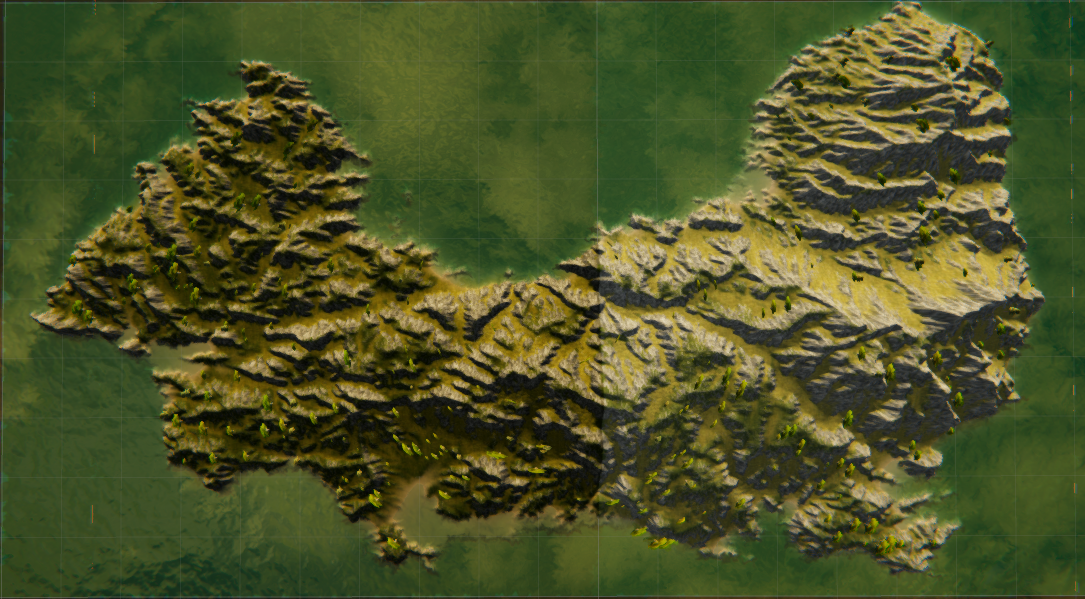
\includegraphics[scale=.3]{Images/island_lookover.png}
    \caption{The 3D model of the  Chios Island (Greece)}
    \label{fig:island}
\end{figure}

The components are also important as the environment itself. Because,  animals , trees , wind and the other factors and components makes the environment a live atmosphere . ( See Fig.\ref{fig:rabbit} , Fig.\ref{fig:deer_herd} and Fig.\ref{fig:bird_flock_fly}) . 



All the 3D object has LOD (Level of Detail) optimization to be rendered in the camera includes the terrain of the environment.

There is 4 different kinds of tree , 4 different kinds of bush and flowers , 3 different kind of grass , 3 different kinds of grass texture and 2 different kinds of stone and rocks used in the whole simulatioon . Most of the used assets taken from the Unitys assets store .

\newpage

\begin{figure}[ht]
    \centering
    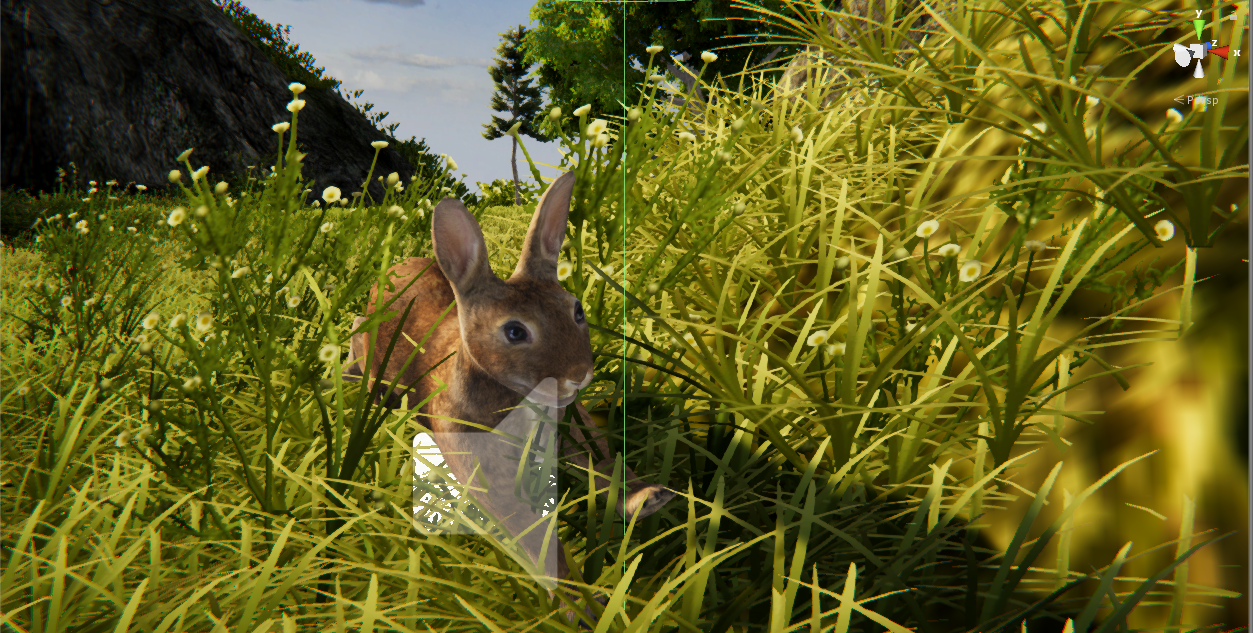
\includegraphics[scale=.26]{Images/rabbit_.png}
    \caption{AI Implemented Rabbit}
    \label{fig:rabbit}
\end{figure}

\begin{figure}[ht]
    \centering
    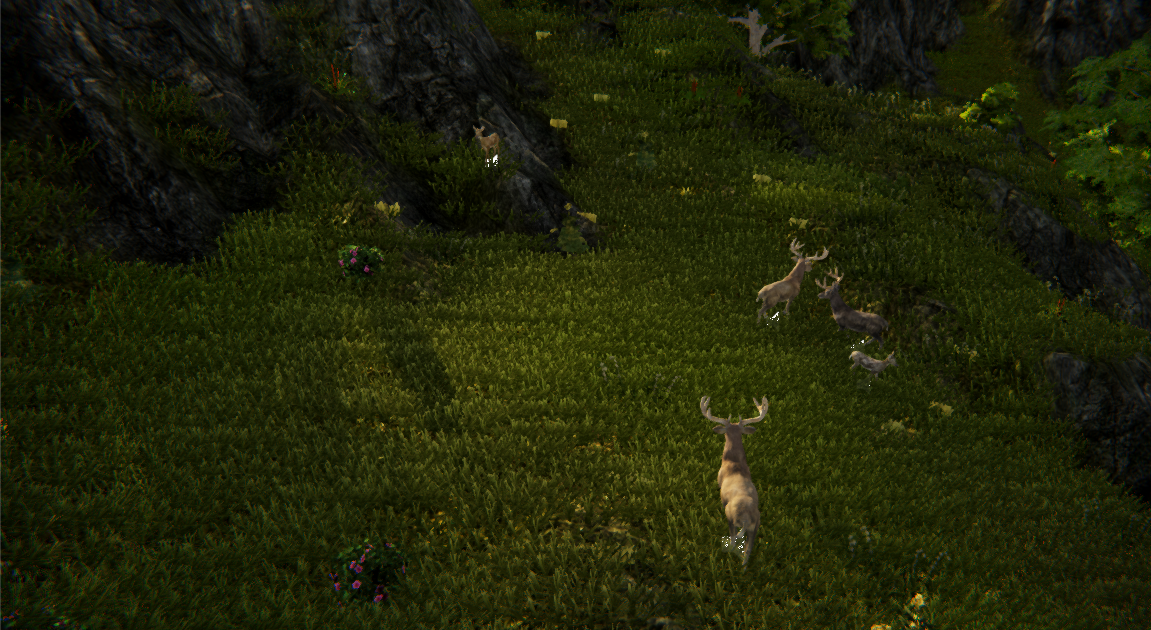
\includegraphics[scale=.285]{Images/deers_AI.png}
    \caption{AI Implemented Deer Herd}
    \label{fig:deer_herd}
\end{figure}

\begin{figure}[ht]
    \centering
    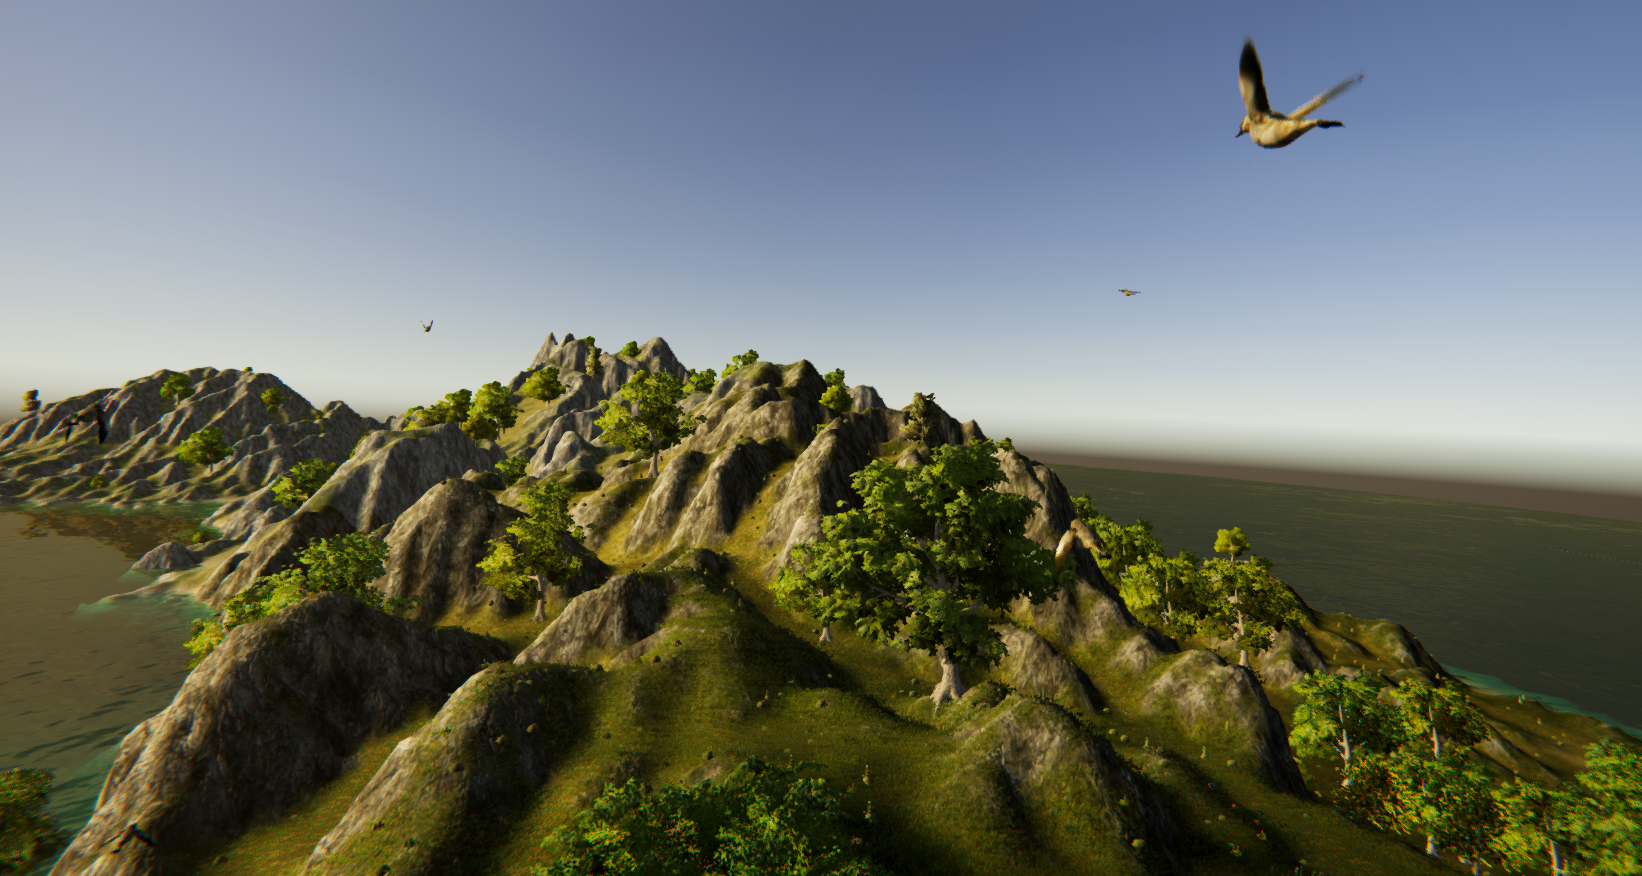
\includegraphics[scale=.202]{Images/birds_flock.png}
    \caption{Flying With the Implemented Birds Flock}
    \label{fig:bird_flock_fly}
\end{figure}
